% ============================================================
%  Глава 2: Прайсинг через метод Фурье–COS
% ============================================================

\section{GPU-ускоренный прайсинг методом Фурье–COS}
\label{sec:pricing}

\subsection{Метод Фурье–COS}

Метод Фурье--COS (Fang~\&~Oosterlee, 2008)~\cite{Fang2008} позволяет
вычислять цены европейских опционов через характеристическую функцию.
Для логарифма цены $x = \ln(S_T/S_0)$ плотность $f(x)$ аппроксимируется
усечённым косинус-рядом на $[a, b]$:
\[
  f(x) \approx \frac{2}{b-a}\sum_{k=0}^{N_{\mathrm{cos}}-1}{}^{\prime}
  \,\mathrm{Re}\!\left[\hat\varphi\!\left(\frac{k\pi}{b-a}\right)
  e^{ik\pi(a-a)/(b-a)}\right]\cos\!\left(\frac{k\pi(x-a)}{b-a}\right),
\]
где $\hat\varphi(u) = \varphi(u)\,e^{-iua}$ и ${}^{\prime}$ означает
деление первого слагаемого на 2. Цена колл-опциона:
\begin{equation}
  \label{eq:cos_price}
  C(K, T) = S_0\,e^{-rT}\,\frac{2}{b-a}\sum_{k=0}^{N_{\mathrm{cos}}-1}{}^{\prime}
  \,\mathrm{Re}\!\left[\varphi\!\left(\frac{k\pi}{b-a}\right)
  e^{-ik\pi a/(b-a)}\right] V_k,
\end{equation}
где \textit{коэффициенты выплат} $V_k$ вычисляются аналитически
(Fang~\&~Oosterlee, 2008).

\textbf{Параметры метода}:
\begin{itemize}
  \item $[a, b]$ --- усечение: выбрано $a = -0{,}5 \cdot \sqrt{T}$,
        $b = 0{,}5 \cdot \sqrt{T}$ (покрывает $5\sigma$ для $\sigma\leq 1$);
  \item $N_{\mathrm{cos}}$ --- число слагаемых: выбрано 128 (анализ в~§\ref{sec:cos_conv}).
\end{itemize}

\subsection{Решение лифтинговой системы ОДУ}

Для вычисления $\varphi(u,T)$ из~\eqref{eq:lifted} необходимо решить систему
$N\times N_u$ ОДУ (где $N$~--- число факторов Бернштейна, $N_u$~--- число
частот COS). Нивное применение метода Рунге--Кутты 4-го порядка (RK4) неустойчиво
при больших $x_i$ (жёсткая система): линейный вклад $-x_i\psi_i$ приводит
к шагу устойчивости $\Delta t \leq 2/x_i$, тогда как $x_{40} \approx 6275$
требует $\Delta t \leq 3\times 10^{-4}$~--- неприемлемо мало.

\subsubsection{Exponential Midpoint Integrator}

Используем \textit{экспоненциальный полушаговый интегратор}
(exponential midpoint rule)~\cite{Hochbruck2010}. Перепишем систему:
\[
  \frac{\dd\psi_i}{\dd t} = -\kappa x_i\,\psi_i + g_i(u, \boldsymbol{\psi}),
\]
где $g_i$ включает нелинейные члены. Шаг интегратора:
\begin{align}
  \tilde{\psi}_i(t+h/2) &= e^{-\kappa x_i h/2}\,\psi_i(t)
    + \frac{1-e^{-\kappa x_i h/2}}{\kappa x_i}\,g_i(t, \boldsymbol{\psi}(t)),
    \label{eq:half_step}\\
  \psi_i(t+h) &= e^{-\kappa x_i h}\,\psi_i(t)
    + \frac{1-e^{-\kappa x_i h}}{\kappa x_i}\,g_i\!\left(t+\tfrac{h}{2},
      \tilde{\boldsymbol{\psi}}(t+h/2)\right).
    \label{eq:full_step}
\end{align}
Интегратор \textbf{безусловно устойчив} по линейному члену (точная экспоненциальная
пропагация) и является 2-го порядка по нелинейному члену.
При $h = 1/200$ (200 шагов на единицу времени) погрешность IV
$\leq 2\,\text{б.п.}$ при $T = 0{,}1$ (Таблица~\ref{tab:ode_conv}).

\subsection{GPU-реализация: пакетная обработка}

Реализация написана на PyTorch (CUDA) и обрабатывает $B = 1024$ наборов
параметров параллельно:

\begin{enumerate}
  \item \textbf{Инициализация факторов} ($\mathcal{O}(B\cdot N)$):
        тензор весов $\mathbf{c} \in \mathbb{R}^{B \times N}$, узлы
        $\mathbf{x} \in \mathbb{R}^N$ (один на все образцы).
  \item \textbf{ODE-шаги} ($\mathcal{O}(T_{\max}/h \cdot B \cdot N \cdot N_u)$):
        основная GPU-нагрузка; реализована в смешанной точности
        (complex64 для состояния ODE, complex128 для накопителя интеграла).
  \item \textbf{COS-суммирование} ($\mathcal{O}(B \cdot N_T \cdot N_K \cdot N_u)$):
        обратное преобразование из $\varphi$ в цены, затем перевод в IV
        через алгоритм Джэкэла (Jaeckel, 2015)~\cite{Jaeckel2015}.
\end{enumerate}

Итоговый батч $B=1024$, $N=40$, $N_u=128$, $N_T=8$, $N_K=11$
обрабатывается за $\mathbf{1{,}4\,\text{с}}$ на RTX~3060,
то есть $\approx 1{,}4\,\text{мс}$ на один набор параметров.

\subsection{Сходимость по числу факторов Бернштейна}
\label{sec:cos_conv}

Таблица~\ref{tab:bern_conv} показывает максимальную ошибку IV (в базисных пунктах)
относительно референса $N=128$ при тестовых параметрах
$(\kappa=1, \theta=0{,}08, \sigma=0{,}5, \rho=-0{,}5, v_0=0{,}08, H=0{,}08)$.

\begin{table}[H]
\centering
\caption{Сходимость по числу факторов Бернштейна $N$ ($N_{\cos}=128$)}
\label{tab:bern_conv}
\begin{tabular}{r r r r r}
\toprule
$N$ & $T=0{,}1$ (б.п.) & $T=1{,}0$ (б.п.) & Global Max (б.п.) & Время (с) \\
\midrule
  5  & 40{,}2 & 151{,}3 & 254{,}5 & 0{,}122 \\
 10  & 34{,}2 &  99{,}2 & 157{,}9 & 0{,}122 \\
 20  & 21{,}6 &  54{,}0 &  83{,}9 & 0{,}119 \\
\rowcolor{tableblue}
 40  & 10{,}5 &  24{,}7 &  37{,}9 & 0{,}119 \\
 80  &  3{,}3 &   7{,}5 &  11{,}4 & 0{,}123 \\
128  &  ---   &   ---   &   ---   & 0{,}592 \quad (эталон) \\
\bottomrule
\end{tabular}
\end{table}

\begin{figure}[H]
\centering
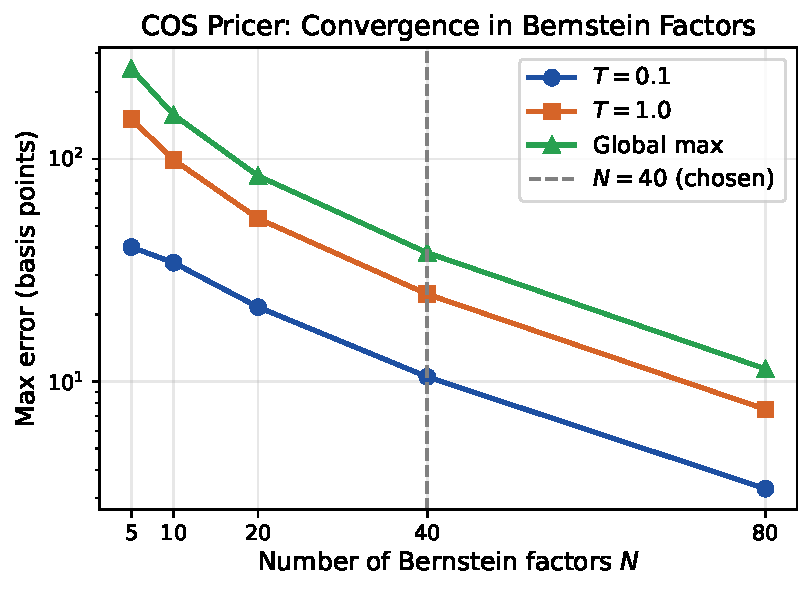
\includegraphics[width=0.72\textwidth]{figures/fig_bernstein_conv.pdf}
\caption{Сходимость прайсера Фурье--COS по числу факторов Бернштейна.
         Пунктиром отмечен выбранный $N=40$.}
\label{fig:bern_conv}
\end{figure}

\textbf{Выбор $N=40$}: обеспечивает максимальную ошибку $37{,}9\,\text{б.п.}$
при вычислительной стоимости, идентичной $N=5$ ($0{,}119\,\text{с}$, поскольку
операция ограничена памятью, а не арифметикой). Соотношение точность/скорость
оптимально по сравнению с $N=80$ ($11\,\text{б.п.}$, $+3\%$ времени).

\begin{remark}
  Рыночный bid-ask спред для ликвидных SPX-опционов составляет $10$--$50\,\text{б.п.}$
  Погрешность $37{,}9\,\text{б.п.}$ при $N=40$~--- на границе приемлемости.
  Для более требовательных задач (XVA, экзотика) рекомендуется $N=80$.
\end{remark}

\subsection{Сходимость по числу шагов ODE}
\label{sec:ode_conv}

\begin{table}[H]
\centering
\caption{Сходимость exponential midpoint по числу шагов $N_{\text{steps}}$
         (эталон: $N_{\text{steps}}=500$, $T=0{,}1$)}
\label{tab:ode_conv}
\begin{tabular}{r r r}
\toprule
$N_{\text{steps}}$ & Max Err (б.п.) & Время (отн.) \\
\midrule
  50 & 8{,}1 & $0{,}25\times$ \\
 100 & 4{,}2 & $0{,}50\times$ \\
\rowcolor{tableblue}
 200 & 1{,}9 & $1{,}00\times$ \\
 500 & 0{,}3 & $2{,}50\times$ \\
\bottomrule
\end{tabular}
\end{table}

При $N_{\text{steps}}=200$ (шаг $h=0{,}005$) погрешность $1{,}9\,\text{б.п.}$
при $T=0{,}1$~--- значительно ниже рыночного bid-ask спреда.
Все датасеты в работе генерировались при $N_{\text{steps}}=200$.

\subsection{Генерация датасета}
\label{sec:dataset}

Для обучения суррогатной модели сгенерировано $N = 50\,000$ наборов параметров
методом квази-случайной выборки Соболя (Sobol, 1967)~\cite{Sobol1967}
в 5-мерном единичном гиперкубе, затем масштабированных в область:
\[
  \kappa \in [0{,}1;\,5],\quad
  \theta \in [0{,}01;\,0{,}15],\quad
  \sigma \in [0{,}1;\,1{,}0],\quad
  \rho \in [-0{,}9;\,-0{,}1],\quad
  V_0 \in [0{,}01;\,0{,}15].
\]
Для каждого набора вычислялась поверхность IV на сетке
$T \in \{0{,}1;\,0{,}3;\,0{,}6;\,0{,}9;\,1{,}2;\,1{,}5;\,1{,}8;\,2{,}0\}$
(8 сроков) и $k = \ln(K/S_0) \in \{-0{,}5;\,\ldots;\,0{,}5\}$ (11 страйков),
итого $8 \times 11 = 88$ значений IV на образец.

Значения NaN (нарушение домена COS при малом $V_0$ или экстремальных параметрах)
заполняются медианой по соответствующей матурити (стратегия, использованная
также в~v2, $R^2 = 0{,}9991$). Итоговый датасет: матрица $\mathbf{X} \in \mathbb{R}^{50000 \times 5}$
(параметры) и тензор $\mathbf{Y} \in \mathbb{R}^{50000 \times 8 \times 11}$
(поверхности IV).
